
\documentclass{article}

\usepackage{arxiv}

\usepackage[utf8]{inputenc} % allow utf-8 input
\usepackage[T1]{fontenc}    % use 8-bit T1 fonts
\usepackage{hyperref}       % hyperlinks
\usepackage{url}            % simple URL typesetting
\usepackage{booktabs}       % professional-quality tables
\usepackage{amsfonts}       % blackboard math symbols
\usepackage{nicefrac}       % compact symbols for 1/2, etc.
\usepackage{microtype}      % microtypography
\usepackage{lipsum}		% Can be removed after putting your text content
\usepackage{graphicx}
\usepackage{natbib}
\usepackage{doi}

% for table with diagonal box
\usepackage{diagbox}

% for writing pusedo-code
\usepackage[algo2e,vlined,ruled]{algorithm2e}

% for code
\usepackage{listings}
\usepackage{color}
\definecolor{dkgreen}{rgb}{0,0.6,0}
\definecolor{gray}{rgb}{0.5,0.5,0.5}
\definecolor{mauve}{rgb}{0.58,0,0.82}
% \lstset{basicstyle=\footnotesize, numbers=left,numberstyle=\tiny, keywordstyle=\color{blue}, frame=single, extendedchars=false, xleftmargin=2em, xrightmargin=2em, aboveskip=1em, showspaces=false, commentstyle=\color{dkgreen}, stringstyle=\color{mauve}}
\lstset{ %
  language=Octave,                % the language of the code
  basicstyle=\scriptsize,           % the size of the fonts that are used for the code
  numbers=left,                   % where to put the line-numbers
  numberstyle=\tiny\color{gray},  % the style that is used for the line-numbers
  stepnumber=1,                   % the step between two line-numbers. If it's 1, each line 
                                  % will be numbered
  numbersep=5pt,                  % how far the line-numbers are from the code
  backgroundcolor=\color{white},      % choose the background color. You must add \usepackage{color}
  showspaces=false,               % show spaces adding particular underscores
  showstringspaces=false,         % underline spaces within strings
  showtabs=false,                 % show tabs within strings adding particular underscores
  frame=single,                   % adds a frame around the code
  rulecolor=\color{black},        % if not set, the frame-color may be changed on line-breaks within not-black text (e.g. commens (green here))
  tabsize=2,                      % sets default tabsize to 2 spaces
  captionpos=b,                   % sets the caption-position to bottom
  breaklines=true,                % sets automatic line breaking
  breakatwhitespace=false,        % sets if automatic breaks should only happen at whitespace
  title=\lstname,                   % show the filename of files included with \lstinputlisting;
                                  % also try caption instead of title
  keywordstyle=\color{blue},          % keyword style
  commentstyle=\color{dkgreen},       % comment style
  stringstyle=\color{mauve},         % string literal style
  escapeinside={\%*}{*)},            % if you want to add LaTeX within your code
  morekeywords={*,...},               % if you want to add more keywords to the set
  xleftmargin=2em,
  xrightmargin=2em,
  aboveskip=1em,
  belowskip=0em
}



% for table
\usepackage{tabularx}
\usepackage{graphicx}
% \usepackage{booktabs}
%  \usepackage{makecell}
 \usepackage{float}
%  \newcommand{\diff}{\,\mathrm{d}}
% \usepackage[margin=1in]{geometry}
% \usepackage{fancyhdr}
% \pagestyle{fancy}
% \usepackage{extarrows}
% \usepackage{breqn}
% % \usepackage[colorlinks,linkcolor=black]{hyperref}
% \usepackage[colorlinks,linkcolor=blue]{hyperref} % 如果想要目录的颜色是蓝色那就用blue
% \newcommand{\N}{\mathbb{N}}
% \newcommand{\Z}{\mathbb{Z}}
% \newcommand{\trans}{^{\mathrm T}}
% \usepackage{amssymb}
% \usepackage[table]{xcolor}
% \usepackage{bm}
% \usepackage{array}
% \usepackage{mathtools}
% \usepackage[english]{babel}
% \usepackage{natbib}
% \usepackage{url}
% \usepackage[utf8x]{inputenc}
% \usepackage{amsmath}
% \graphicspath{{images/}}
% \usepackage{parskip}
% \usepackage{fancyhdr}
% \usepackage{vmargin}
% \usepackage[font={bf, footnotesize}, textfont=md]{caption}
% \usepackage{amsmath,amsthm,amssymb}


% \newenvironment{theorem}[2][Theorem]{\begin{trivlist}
% \item[\hskip \labelsep {\bfseries #1}\hskip \labelsep {\bfseries #2.}]}{\end{trivlist}}
% \newenvironment{lemma}[2][Lemma]{\begin{trivlist}
% \item[\hskip \labelsep {\bfseries #1}\hskip \labelsep {\bfseries #2.}]}{\end{trivlist}}
% \newenvironment{exercise}[2][Exercise]{\begin{trivlist}
% \item[\hskip \labelsep {\bfseries #1}\hskip \labelsep {\bfseries #2.}]}{\end{trivlist}}
% \newenvironment{reflection}[2][Reflection]{\begin{trivlist}
% \item[\hskip \labelsep {\bfseries #1}\hskip \labelsep {\bfseries #2.}]}{\end{trivlist}}
% \newenvironment{proposition}[2][Proposition]{\begin{trivlist}
% \item[\hskip \labelsep {\bfseries #1}\hskip \labelsep {\bfseries #2.}]}{\end{trivlist}}
% \newenvironment{corollary}[2][Corollary]{\begin{trivlist}
% \item[\hskip \labelsep {\bfseries #1}\hskip \labelsep {\bfseries #2.}]}{\end{trivlist}}
% \DeclareMathOperator{\tr}{tr}
% \DeclareMathOperator{\rank}{rank}
% \DeclareMathOperator{\Span}{span}
% \DeclareMathOperator{\row}{row}
% \DeclareMathOperator{\col}{col}
% \DeclareMathOperator{\range}{range}
% \DeclarePairedDelimiterX{\inp}[2]{\langle}{\rangle}{#1, #2}
% \DeclareMathOperator{\Proj}{Proj}
% \DeclareMathOperator{\trace}{trace}
% \newcommand{\Her}{^{\mathrm H}}
% \DeclareMathOperator{\diag}{diag}
% \makeatletter 
%     \newcommand\fcaption{\def\@captype{table}\caption}
% \makeatother
% \setmarginsrb{2.5 cm}{1.5 cm}{2.5 cm}{1.5 cm}{1 cm}{1 cm}{1 cm}{1 cm}


% \makeatletter
% \let\thetitle\@title
% \let\theauthor\@author
% \let\thedate\@date
% \makeatother

% \pagestyle{fancy}
% \fancyhf{}
% \rhead{\theauthor}
% \lhead{\thetitle}
% \cfoot{\thepage}

\title{High-Frequency Statistical Arbitrage}

\date{\today}	% Here you can change the date presented in the paper title
% \date{} 					% Or removing it


\author{Boyu Yang\\The Chinese University of Hong Kong, Shenzhen\\boyuyang@link.cuhk.edu.cn}

% \author{ \href{https://orcid.org/0000-0000-0000-0000}{\includegraphics[scale=0.06]{orcid.pdf}\hspace{1mm}David S.~Hippocampus}\thanks{Use footnote for providing further
% 		information about author (webpage, alternative
% 		address)---\emph{not} for acknowledging funding agencies.} \\
% 	Department of Computer Science\\
% 	Cranberry-Lemon University\\
% 	Pittsburgh, PA 15213 \\
% 	\texttt{hippo@cs.cranberry-lemon.edu} \\
	%% examples of more authors
	% \And
	% \href{https://orcid.org/0000-0000-0000-0000}{\includegraphics[scale=0.06]{orcid.pdf}\hspace{1mm}Elias D.~Striatum} \\
	% Department of Electrical Engineering\\
	% Mount-Sheikh University\\
	% Santa Narimana, Levand \\
	% \texttt{stariate@ee.mount-sheikh.edu} \\
	%% \AND
	%% Coauthor \\
	%% Affiliation \\
	%% Address \\
	%% \texttt{email} \\
	%% \And
	%% Coauthor \\
	%% Affiliation \\
	%% Address \\
	%% \texttt{email} \\
	%% \And
	%% Coauthor \\
	%% Affiliation \\
	%% Address \\
	%% \texttt{email} \\
% }

% Uncomment to remove the date
%\date{}

% Uncomment to override  the `A preprint' in the header
%\renewcommand{\headeright}{Technical Report}
%\renewcommand{\undertitle}{Technical Report}
\renewcommand{\shorttitle}{High-Frequency Statistical Arbitrage}

%%% Add PDF metadata to help others organize their library
%%% Once the PDF is generated, you can check the metadata with
%%% $ pdfinfo template.pdf
\hypersetup{
pdftitle={A template for the arxiv style},
pdfsubject={q-bio.NC, q-bio.QM},
pdfauthor={David S.~Hippocampus, Elias D.~Striatum},
pdfkeywords={First keyword, Second keyword, More},
}



\begin{document}
\maketitle

\begin{abstract}
	The performance of 5G network is highly sensitive to delays. The design of 5G network requires more accurate evaluation on delay distribution. This research aims to accurately measure expected steady-state waiting time and percentile delays of the queueing networks with routing schedules of different levels of complexity. Specifically, non-preemptive priority queue, weighted fair queueing system, and deficit round robin 
	will be simulated using adaptive cross-entropy and importance sampling techniques. Numerical experiments show that our algorithm outperforms benchmark simulation methods. The results mainly contribute to the literature on rare event simulation for queueing systems.
\end{abstract}


% keywords can be removed
\keywords{Statistical Arbitrage \and Pairs Trading \and High-Frequency Trading \and Ornstein-Uhlenbeck Process}


\section{Introduction}
The performance of 5G network is highly sensitive to delays. The design of 5G network requires more accurate evaluation on delay distribution. The project aims to develop fast simulation algorithms to evaluate tail probability and percentile of delay, which are known as service level agreement (SLA) in communication networks. 
	The simulator is constructed using queueing theory and algorithm is designed using importance sampling techniques.

In the following simulation, random seed is set to be 43 to ensure the results are reproduceable.

\section{Literature Review}


\section{Data Manipulations}

\subsection{Data Source}


\subsection{Data Processing}


\section{Proposed Model}



\section{Model Validation}



\section{Conclusion}


\section{Notation}
The notations that will be used is summarized in the table.
\begin{table*}[!htbp]
    
	\centering
	\begin{tabularx}{0.55\textwidth}{cl}
		\toprule
        \textbf{Attribute}
		&  \textbf{Description} \\
		\midrule
		$W_n$ 
		& Waiting time of the $n$th customer 
		\\
		\midrule
		$V_n$ 
		& Service time of the $n$th customer
        \\
        \midrule
        $T_n$
        & Interarrival time of the $n$th customer
        \\
        \midrule
        $\sigma$
        & Cycle length of the regenerative cycle
        \\
        \midrule
        $\tau$
        & The first time that {$W_n$} exceeds a threshold $\gamma$
        \\
		\bottomrule
	\end{tabularx}%
	\label{tab:addlabel}%
	\caption{A table of notations description}
\end{table*}%



\section{M/M/1 First-in-First-out Queue}
\label{sec:headings}
For the simplest M/M/1 queue, the expected waiting time and tail probability have analytical solutions. With independent poisson arrival (rate $\lambda$) and exponential service time (rate $\mu$) assumption, the expected waiting time is given by ${\rm E}[W_{\infty}]=\rho / (\mu - \lambda)$ and the tail probability is given by $P(W_{\infty}>\gamma)=\rho \times e^{-(\mu - \lambda)\gamma}$.
We consider a single case of $\lambda = 1.5,\mu = 2$ for the first two methods and two cases of light and heavy traffic for the change of measure method.
% \lipsum[4] See Section \ref{sec:headings}.

\subsection{Direct Simulation by Lindley Recursion}
Consider a single-server queue possessing an infinite capacity waiting room and processing customers according to "first-in-first-out" routing schedule. Let $W_n$, $V_n$, $T_n$ be the waiting time, service time, and interarrival time for the $n$th customer to enter the queue. By the \emph{Lindley Recursion} formula \citep{asmussen2007stochastic}, we have

\begin{equation}
	W_{n+1}=[W_n+V_n-T_n]^{+}
\end{equation}

In an M/M/1 queue, $T_n$, $V_n$ follow i.i.d exponential distributions with rate $\lambda$ and $\mu$ respectively. Hence we can directly simulate the dynamics of the M/M/1 queue using random number generator in Python. 
The estimation for the waiting time expectation is calculated by Crude Monte Carlo (CMC). 
The 95\% normal confidence interval is given by ${\rm \hat{E}}[W_n] \pm  1.96\times \sigma_{{\rm \hat{E}}[W_n]} / n^{1/2}$.
We get the simulation mean and 95\% confidence intervals for $E[W_n]$ with $n=1,10,100,1000,10000$ where $\lambda = 1.5$ and $\mu = 2$ in table 2. 


\begin{table*}[!htbp]
    \small
	\centering
	\begin{tabularx}{0.4\textwidth}{rcc}
		\toprule
        n
		& $\hat{{\rm E}}[W_n]$ 
        & 95\% CI
		\\

        \midrule
        1
        & 0.000000
        & [0.000000, 0.000000]
		

        \\
        \midrule
        10
        & 0.854324
        & [0.844877, 0.863772]
		

        \\
        \midrule
        100
        & 1.483175
        & [1.466490, 1.499860]
		
        \\
        \midrule
        1000
        & 1.504443 
        & [1.487524, 1.521363]
		
		\\
        \midrule
        10000
        & 1.509648
        & [1.492566, 1.526730]
        \\
		\bottomrule
	\end{tabularx}%
	\label{tab:tab1}%
	\caption{Simulation by Lindley recursion}
\end{table*}%

Since the theoretical result of the steady state mean waiting time is $\rho/{(\mu - \lambda)}$, in which case is 1.5 for the accurate value, we can see from the simulation result that when the system is runned for a long time, the expected mean waiting time is becoming closer to the true value. 

We generate 50000 sample paths for each case to ensure the width of confidence intervals to be smaller than 0.05. For all the cases above, the 95\% confidence intervals with width smaller than 0.05 cover the true value of 1.5.
However, for other random seeds tried, the result and the confidence intervals are fluctuating, sometimes cover the true value but sometimes may not. This indicates simulating the steady-state distribution simply by running the system for a long time may be inaccurate since the relative error is large. Also the simulation takes plenty of time in order to stabilize the performance of CMC method especially when $n$ is large.


\subsection{Simulation Using Regenerative Method}
A general M/G/1 queue possesses the behavior that at each time point when a customer arrives at an empty system, the process probabilistically restart itself \citep{rubinstein2016simulation}. Let $\sigma_i$ be the i.i.d length of the ith cycle of the regenerative process {$X_t$}. 
\begin{equation}
	\sigma = {\rm inf}\left[n>1|W_n=0\right]-1
\end{equation}

Suppose we want to estimate the steady-state expectation $E[W(X)]$, the regenerative method gives a way to approximate using the following formula.
\begin{equation}
	R_i = \sum_{t=T_{i-1}}^{T_i-1}W(X_t)
\end{equation}
\begin{equation}
	l = {\rm E}[W(X)] = \frac{{\rm E}[R]}{{\rm E}[\sigma]}
\end{equation}
Then we can generate $N$ regenerative cycles, calculate the i.i.d sequence of two-dimensional random vectors ($R_i,\sigma_i$), $i=1,2,\dots,N$, and then use CMC to obtain a point estimate:
\begin{equation}
	\hat{l} = \frac{\hat{R}}{\hat{\sigma}}
\end{equation}
where $\hat{R}=N^{-1}\sum_{i=1}^N R_i$ and $\hat{\sigma}=N^{-1}\sum_{i=1}^N \sigma_i$. The regenerative estimator is biased, namely, $E[\hat{l}] \neq l$. However $\hat{l}$ is strongly consistent by applying the law of large numbers to the numerator and denominator respectively. 
A 95\% confidence interval for the point estimator is given by 
\begin{equation}
	(\hat{l} \pm 1.96\times \frac{S}{\hat{\sigma}N^{1/2}}),
\end{equation}
where
\begin{equation}
	S^2 = \frac{1}{N-1}\sum_{i=1}^N (R_i-\hat{R})^2 - 2\times \hat{l} \times  \frac{1}{N-1}\sum_{i=1}^N (R_i-\hat{R})(\sigma_i-\hat{\sigma}) + \hat{l}^2\times \frac{1}{N-1}\sum_{i=1}^N (\sigma_i-\hat{\sigma})^2
\end{equation}
Using the above formula, we can design the simulation algorithm to get the estimation result for the expected waiting time in an M/M/1 queue in table 3.

\begin{table*}[!htbp]
    \small
	\centering
	\begin{tabularx}{0.47\textwidth}{cccc}
		\toprule
        N
		& $\hat{{\rm E}}[W_n]$ 
        & 95\% CI
		& Theory\\

        \midrule
        1000000
        & 1.498611
        & [1.485029, 1.512194]
		& 1.50

        \\
		\bottomrule
	\end{tabularx}%
	\label{tab:addlabel}%
	\caption{Simulation by regenerative method}
\end{table*}%
We use a large number of cycles to ensure the consistency property of the regenerative method estimator is utilized to the utmost. The result tends to be much more stable and accurate than the previous. The 95\% confidence interval covers the true value 1.5 and the estimated expectation is very close to the true value. 
Though the result is much more accurate, we still need to simulate for a large number of cycles to utilize the consistency property. If the cycle number generated is small (e.g. less than 10000), the estimation is not stable as well and the relative error is still very large.

% \paragraph{Paragraph}
% \lipsum[7]

\subsection{Simulation Using Change of Measure}
Substituting the estimation target of expected steady-state waiting time by the steady-state tail probability, namely, $P(W_{\infty} > \gamma)$, where $\gamma$ is a threshold that is much larger than the expected value $E[W_n]$. This tail probability has practical intuitions in the 5G network. The 5G communication network requires high efficiency to deal with tasks of different packet sizes. If the waiting time of a single packet exceeds a threshold, the whole communication network may become jammed, which may cause devastating effects to the whole system. 
Hence we need more fast and low error estimation methods to accurately measure the tail probability.

By the previous regenerative method, the tail probability satisfies
\begin{equation}
	P(W_{\infty}>\gamma)=\frac{{\rm E}[\sum_{n=1}^{\sigma}I(W_n \geq \gamma)]}{{\rm E}[\sigma]}	
\end{equation}
Hence the tail probability can be estimated directly using direct CMC method. However, due to the large relative error, we seek to improve the accuracy and lower down the estimation variance using importance sampling \citep{ross2014introduction}.

\subsubsection{Importance Sampling}
Now we present the method of importance sampling in M/G/1 network \citep{rubinstein2004cross}.
Denote the first time that {$W_n$} exceeds level $\gamma$ to be $\tau$, then
\begin{equation}
	\tau = {\rm inf} \left[n>1, W_n \geq \gamma\right]
\end{equation}
Consider the following switching change of measure
\begin{equation}
	T_n \sim f^{T} \rightarrow \tilde{f}^{T}\quad {\rm and} \quad V_n \sim g^{V} \rightarrow \tilde{g}^{V}, \quad {\rm for\ } n=1,2,\dots min(\tau, \sigma).    
\end{equation}
Initially we use the IS densities for $V_n$ and $T_n$ until the process {$W_n$} exceeds level $\gamma$, after which we switch back to the original densities. By switching like this the whole process returns to the regenerative state.
The likelihood ratio satisfies
\begin{equation}
	L_n=\left\{
		\begin{array}{lcl}
		L_{n-1}\frac{f^T(T_n)g^V(V_n)}{\tilde{f}^T(T_n)\tilde{g}^V(V_n)}       &      & {n\leq min(\tau, \sigma)}\\
		L_{\tau}     &      & {n\geq min(\tau, \sigma)}
	\end{array} \right.
\end{equation}
 Therefore we can obtain the new formula for estimating the tail probability
 \begin{equation}
	 \ell = P(W_{\infty}>\gamma)=\frac{{\rm E_{w}}[\sum_{n=1}^{\sigma}I(W_n \geq \gamma)]}{{\rm E}[\sigma]}=\frac{{\rm E_{w^{\prime}}}[\sum_{n=1}^{\sigma}I(W_n \geq \gamma)L_n]}{{\rm E}[\sigma]}
 \end{equation}
where the notation $w^{\prime}$ represents the switched distribution under change of measure. 

\subsubsection{M/M/1 Queue Results}
In M/M/1 queue, we switch the rate of interarrival time from $\lambda$ to $\lambda + \theta$ and the rate of service time from $\mu$ to $\mu - \theta$. The optimal parameter value occurs when $\theta^{*} = \mu -\lambda$. We try both the optimal $\theta$ and other values of $\theta$ that are near the optimal value to obtain more insights.

By using Monte Carlo estimation separately for numerator and denominator, we obtain the estimation results as the following table. It should be noted that the 95\% confidence interval for the numerator is the usual normal confidence interval, and the 95\% confidence interval for the whole probability is calculated using the same formula as equation (6). 
The relative error is calculated using $\sigma_{IS}/l$ where $l$ is the estimation expectation. The number of cycles is fixed to be $10^5$ and the time for simulation is measured. 
\begin{table*}[!htbp]
    \tiny
	\centering
	\begin{tabularx}{1.07\textwidth}{cccccccccccc}
		\toprule
        $\theta$
		& $\frac{\lambda}{\lambda + \theta} \frac{\mu}{\mu - \theta}$
		& $\gamma$
		& Theory
		& Num Mean
		& Num 95\% CI
		& Num\_RE
		& Prob Mean
		& Prob 95\% CI
		& Prob\_RE
		& Cycle Num
        & Time\\

        \midrule
        1.6348
        & 0.9
        & 3.2273
		& 1e-3
		& 0.001498
		& [0.001481, 0.001516]
		& 0.00587
		& 0.001002
		& [0.000989, 0.001015]
		& 0.00667
		& 1e5
		& 9.6s

        \\
        \midrule
        1.8
        & 1
        & 3.2273
		& 1e-3
		& 0.001495
		& [0.001478, 0.001510]
		& 0.005498
		& 0.00099967
		& [0.000987, 0.001012]
		& 0.006355
		& 1e5
		& 9.7s
        \\
		
        \midrule
        1.91534
        & 1.1
        & 3.2273
		& 1e-3
		& 0.001496
		& [0.001478, 0.001513]
		& 0.005899
		& 0.00099945
		& [0.000986, 0.001012]
		& 0.006701
		& 1e5
		& 9.7s
        \\
		\midrule
        1.6348
        & 0.9
        & 5.78573
		& 1e-5
		& 1.5076e-05
		& [1.4893e-05, 1.5260e-05]
		& 0.006210
		& 1.00413e-05
		& [9.9039e-06, 1.0179e-05]
		& 0.006979
		& 1e5
		& 14.9s
        \\
		\midrule
        1.8
        & 1
        & 5.78573
		& 1e-5
		& 1.5066e-05
		& [1.4905e-05, 1.5227e-05]
		& 0.005440
		& 1.00067e-05
		& [9.8831e-06, 1.0130e-05]
		& 0.006306
		& 1e5
		& 14.8s
        \\
		\midrule
        1.91534
        & 1.1
        & 5.78573
		& 1e-5
		& 1.5015e-05
		& [1.4835e-05, 1.5195e-05]
		& 0.006112
		& 9.9763e-06
		& [9.8418e-06, 1.0111e-05]
		& 0.006878
		& 1e5
		& 14.5s
        \\
		\midrule
        1.6348
        & 0.9
        & 12.1818
		& 1e-10
		& 1.4980e-10
		& [1.4767e-10, 1.5193e-10]
		& 0.007255
		& 9.95643e-11
		& [9.8020e-11, 1.0111e-10]
		& 0.007913
		& 1e5
		& 28.7s
        \\
		\midrule
        1.8
        & 1
        & 12.1818
		& 1e-10
		& 1.4821e-10
		& [1.4663e-10, 1.4979e-10]
		& 0.005448
		& 9.85027e-11
		& [9.7288e-11, 9.9718e-11]
		& 0.006293
		& 1e5
		& 27.8s
        \\
		\midrule
        1.91534
        & 1.1
        & 12.1818
		& 1e-10
		& 1.5049e-10
		& [1.4844e-10, 1.5255e-10]
		& 0.006999
		& 1.00299e-10
		& [9.8788e-11, 1.0181e-10]
		& 0.007683
		& 1e5
		& 26.1s
        \\
		\bottomrule
	\end{tabularx}%
	\label{tab:tab4}%
	\caption{Simulation by Change of Measure: Light Traffic ($\lambda = 0.9, \mu = 2.7$)}
\end{table*}%

\begin{table*}[!htbp]
    \tiny
	\centering
	\begin{tabularx}{1.09\textwidth}{cccccccccccc}
		\toprule
        $\theta$
		& $\frac{\lambda}{\lambda + \theta} \frac{\mu}{\mu - \theta}$
		& $\gamma$
		& Theory
		& Num Mean
		& Num 95\% CI
		& Num\_RE
		& Prob Mean
		& Prob 95\% CI
		& Prob\_RE
		& Cycle Num
        & Time\\

        \midrule
        0.28761
        & 0.99
        & 16.7115
		& 1e-3
		& 0.00493
		& [0.0047, 0.00510]
		& 0.020451
		& 0.00099
		& [0.00099, 0.00103]
		& 0.020676
		& 1e5
		& 48.4s

        \\
        \midrule
        0.4
        & 1
        & 16.7115
		& 1e-3
		& 0.00503
		& [0.0049, 0.00515]
		& 0.012286
		& 0.0009975
		& [0.00097, 0.001022]
		& 0.012635
		& 1e5
		& 59.7s
        \\
		
        \midrule
        0.7752
        & 1.1
        & 16.7115
		& 1e-3
		& 0.00396
		& [0.00326, 0.00465]
		& 0.089492
		& 0.000795
		& [0.00065, 0.00093]
		& 0.089551
		& 1e5
		& 1m25.3s
        \\
		\midrule
        0.28761
        & 0.99
        & 28.2244
		& 1e-5
		& 5.00243e-05
		& [4.7239e-05, 5.2809e-05]
		& 0.028402
		& 9.96397e-06
		& [9.4056e-06, 1.0522e-05]
		& 0.028587
		& 1e5
		& 1m18.2s
        \\
		\midrule
        0.4
        & 1
        & 28.2244
		& 1e-5
		& 4.96383e-05
		& [4.8433e-05, 5.0843e-05]
		& 0.012381
		& 9.92358e-06
		& [9.6746e-06, 1.0172e-05]
		& 0.012796
		& 1e5
		& 1m39.4s
        \\
		\midrule
        0.7752
        & 1.1
        & 28.2244
		& 1e-5
		& 3.50894e-05
		& [1.32093e-05, 5.6969e-05]
		& 0.318137
		& 7.02506e-06
		& [2.64424e-06, 1.1406e-05]
		& 0.318162
		& 1e5
		& 2m17.7s
        \\
		\midrule
        0.28761
        & 0.99
        & 57.0067
		& 1e-10
		& 4.6518e-10
		& [4.2200e-10, 5.0836e-10]
		& 0.047354
		& 9.3716e-11
		& [8.49982e-11, 1.024e-10]
		& 0.047462
		& 1e5
		& 2m55.4s
        \\
		\midrule
        0.4
        & 1
        & 57.0067
		& 1e-10
		& 5.0849e-10
		& [4.9623e-10, 5.2074e-10]
		& 0.012294
		& 1.02568e-10
		& [1.0001e-10, 1.0512e-10]
		& 0.012703
		& 1e5
		& 3m44.9s
        \\
		\midrule
        0.7752
        & 1.1
        & 57.0067
		& 1e-10
		& 2.65308e-10
		& [8.6503e-12, 5.2190e-10]
		& 0.493568
		& 5.31031e-11
		& [1.7280e-12, 1.0447e-10]
		& 0.493593
		& 1e5
		& 5m39.5s
        \\
		\bottomrule
	\end{tabularx}%
	\label{tab:tab5}%
	\caption{Simulation by Change of Measure: Heavy Traffic ($\lambda = 1.6, \mu = 2$)}
\end{table*}%
It can be easily seen that in most cases, the 95\% confidence interval covers the theoretical value, and the estimated mean is close to the true value. However, in the heavy traffic cases, some choices of $\theta$ fail to give an accurate estimate and their confidence intervals do not cover the true value. We leave it in the discussion below.

\subsection{Conclusion}
In the above sections, different simulation techniques have been used to simulate the expected waiting time and tail probability of an M/M/1 queue. We summarize some important insights below.

\paragraph{Lindley Recursion}
Lindley recursion gives a direct recursive way to simulate the waiting time sequence. However, directly running simulations to obtain point estimates for ${\rm E}[W_n]$ for a large value of $n$ to approximate 
the steady-state performance is inaccurate. The results and confidence intervals fluctuate with different random seeds and are not stable due to a large relative error. It also takes plenty of time to generate i.i.d samples of $W_n$ in order to use the Monte Carlo method.

\paragraph{Regenerative Method}
Regenerative method obtains a consistent estimator for the evaluated expectation. When the number of cycles generated is large, the consistency principle can be utilized and the estimated waiting time expectation is very close to the actual value. 
The simulation takes much less time to finish the estimation, but the high relative error problem still exists. This means if the number of cycles generated is relatively small, the obtained point estimate will have large variance and may be inaccurate.

\paragraph{Change of Measure}
By using proper change of measure, the relative error is reduced effectively. However, the performance among different changes of measure differ a lot. We discuss the results by comparing the performance in both the light traffic case and heavy traffic case below:
\begin{itemize}
	\item In most of the cases, using change of measure presents better point estimate and confidence intervals. As shown in the table, the mean of probability estimate is close to the actual value and the 95\% confidence interval covers the theoretical value in most cases.
	\item Different changes of measure obtain similar result of the numerator as well as the estimated probability. Indeed the numerator estimation should be unbiased for different changes of measure.
	\item When the threshold $\gamma$ increases, the probability becomes harder to estimate and the algorithm takes longer time to finish. This makes sense since we will switch back to the original densities only when the "rare event" occurs. When $\gamma$ becomes larger, the "rare event" occurs with much lower probability.
	\item The best change of measure always give the lowest relative error. Taking values of $\theta$ near the optimal value will all increase the relative error. This means even if in the current case (random seed is 43) the algorithm performs better than the optimal change of measure, it may underperform if the random seed is changed.
	\item Improper changes of measure hurt the performance of the algorithm, even worse than the simulation without change of measure. As shown in the table 5, in the heavy traffic case, when the second column is 1.1, the value of $\theta$ actually differ from the optimal parameter (0.4) a lot. It can be easily seen that the corresponding cases ($\theta = 0.7752$) have extremely large relative errors, even hundred times larger than the optimal cases. The estimated value is biased, and the confidence interval fails to cover the true probability.
	\item The heavy traffic case is far more difficult to estimate than the light traffic case. In the algorithm above, simulation for the heavy traffic cases take several times longer than the light traffic cases. Also the tail probability estimation for the light traffic case is more accurate than that of the heavy traffic case. The heavy traffic cases take much longer time and have larger relative error.
\end{itemize}



\section{M/M/1 Non-preemptive Priority Queue}
Now we study the same M/M/1 queueing system, however with different routing principle, i.e. the priority queue. We study the nonpreemptive priority queue, meaning the ongoing service cannot be terminated even if a customer with higher priority comes along. Denote the arrival rates of the $k$ types of customers to be $\lambda_1,\lambda_2,\dots ,\lambda_k$ and the service rates are $\mu_1, \mu_2, \dots, \mu_k$ respectively. The target again is to estimate 1) expected waiting time in steady states, i.e. ${\rm E}[W_{\infty}^{(k)}]$, and 2) tail probability $P(W_{\infty}^{(k)}>\gamma)$ for type k customers. 
\begin{figure}[H]
	\centering
	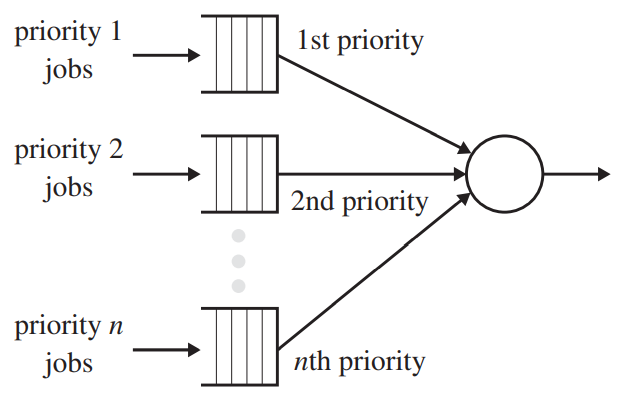
\includegraphics[height=4.4cm]{./figures/priority.png}
	\caption{M/M/1 priority queue illustration}
	\label{fig:fig1}
\end{figure}
We use event-based simulation to construct the algorithm. In the first step direct simulation will be constructed to simulate finite-step waiting time expectation ${\rm E}[W_n^{(k)}]$, then regenerative method and possible changes of measure will be used to estimate the tail probability. It is worth mentioning that in the non-preemptive priority queue case, the expected waiting time has analytical solutions though the best change of measure does not.

\subsection{Event-Based Simulation}

Consider discrete event systems with finitely many components and each component has only finite number of states. Each event takes place at a particular time but has no duration. The system dynamics (or called environment) can be modeled as combinations of upcoming events, with their corresponding time and action. The components of the system interact through different types of events. 

In the nonpreemptive priority queueing system, the components are coming customers and the server. Customers arrive, keep line in a waiting queue, get served, and leave after finishing their services. Hence, the components interact with the environment through three types of events including "arrival", "starting service", and "departure". If a customer arrives, the components will add an event of type "arrival" to the environment. The environment then checks whether the server is free to determine whether to send the instructions of starting service to the server. After starting service, the server state will be set busy and a "departure" type event will be sent to the environment after the service time. 
After the departure of the current customer, the server state is set free again to serve the next potential customer.

\subsection{Direct Simulation of Expected Waiting Time}
\subsubsection{Theoretical Results}
We first present the analytical solutions of the steady-state waiting time \citep{harchol2013performance}.
Assume customers of the first type have the highest priority. Let $V_k$ be the service time of priority $k$ customers.  
Assume the service utilization rate is smaller than 1, that is 
\begin{equation}
	\rho = \sum_{i=1}^n \rho_i = \sum_{i=1}^n \lambda_i {\rm E}[T_i] = \sum_{i=1}^n \frac{\lambda_i}{\mu_i} < 1
\end{equation}
Use ${\rm E}[V_e]$ to represent the expected remaining time of the currently served customer given that there is one customer in service. Then ${\rm E}[V_e]$ is given by
\begin{equation}
	{\rm E}[V_e] = \frac{{\rm E}[V^2]}{2{\rm E}[V]} = \frac{\sum_{i=1}^n p_k {\rm E}[V_k^2] }{2\sum_{i=1}^n p_k{\rm E}[V_k]}=\frac{\sum_{i=1}^n \frac{\lambda_k}{\sum_i \lambda_i}\times \frac{2}{\mu_k^2}}{2\sum_{i=1}^n \frac{\lambda_k}{\sum_i \lambda_i}\times \frac{1}{\mu_k}}
\end{equation} 
Then the expected steady-state waiting time for type-k customers is
\begin{equation}
	{\rm E}[W_{\infty}^{(k)}] = \frac{\rho {\rm E}[V_e]}{(1-\sum_{i=1}^k \rho_i)(1-\sum_{i=1}^{k-1}\rho_i)}
\end{equation}

\subsubsection{Simulation Results}
We start the simulation of the two-class case, where $\lambda_1 = 0.6,\lambda_2 = 0.2$ and $\mu_1 = 2, \mu_2 = 1$. 
Then by the previous formula, the theoretical results will be 
\begin{equation}
	{\rm E}[W_{\infty}^{(1)}]=\frac{\rho {\rm E}[V_e] }{1-\rho_1}
\end{equation}
\begin{equation}
	{\rm E}[W_{\infty}^{(2)}]=\frac{\rho {\rm E}[V_e] }{(1-\rho_1)(1-\rho_1-\rho_2)}
\end{equation}
which is 0.5 for ${\rm E}[W_{\infty}^{(1)}]$ and 1 for ${\rm E}[W_{\infty}^{(2)}]$.
The simulated mean and 95\% normal confidence interval for fixed $n=2, 10, 100, 1000, 10000$ are given in the table (we start with $n=2$ to ensure neither of the waiting time is always 0).
For every fixed $n$, We simulate more than 10000 distinctive paths to make sure the performance of CMC method is stable and the width of the confidence intervals is small enough.

\begin{table*}[!htbp]
    \small
	\centering
	\begin{tabularx}{0.85\textwidth}{rcccccc}
		\toprule
        n
		& $\hat{{\rm E}}[W_n^{(1)}]$ 
		& Theory\_1
        & 95\% CI of $\hat{{\rm E}}[W_n^{(1)}]$
		& $\hat{{\rm E}}[W_n^{(2)}]$ 
		& Theory\_2
		& 95\% CI of $\hat{{\rm E}}[W_n^{(2)}]$
		\\

        \midrule
        2
        & 0.283049
		& 0.50
        & [0.27063, 0.29546]
		& 0.409035
		& 1.00
		& [0.38948, 0.42858]

        \\
        \midrule
        10
        & 0.493606
		& 0.50
        & [0.47668, 0.51053]
		& 0.978137
		& 1.00
		& [0.94036, 1.01591]

        \\
        \midrule
        100
        & 0.500234
		& 0.50
        & [0.48332, 0.51714]
		& 1.020193
		& 1.00
		& [0.98099, 1.05939]
        \\
        \midrule
        1000
        & 0.501783
		& 0.50
        & [0.48485, 0.51871]
		& 1.022466
		& 1.00
		& [0.98400, 1.06092]
		\\
        \midrule
        10000
        & 0.50695
		& 0.50
        & [0.48967, 0.52424]
		& 1.029759
		& 1.00
		& [0.99018, 1.06933]
        \\
		\bottomrule
	\end{tabularx}%
	\label{tab:tab7}%
	\caption{Direct event-based simulation results}
\end{table*}%

Compared with the theoretical results (0.5 and 1), we can see the simulation results for both classes are very close to the true value. Except for the case when $n=2$, all other scenarios have their 95\% confidence intervals covered the true parameter value, though simulations with large value of $n$ take extremely long time to finish.
In later sections we will explore possible changes of measure and use regenerative method again to obtain more fast and accurate simulation algorithms.


\subsubsection{Some Insights}

From the table, customers with higher priority have smaller expected waiting time than those with lower priority. It can be expected that if the priority queue is preemptive, then those customers with higher priority will have even smaller expected waiting time. 

Besides, the numerator of the expected waiting time formula is the same, regardless of which type the customer belongs to. This term is due to waiting for the customer that is currently served, which equals the probability that there is one customer in the service ($\rho$) multiply by the expected remaining time on that customer given that there is a customer in the service (${\rm E}[V_e]$). 
The denominator, however, decreases as the priority decreases. The term ($1-\sum_{i=1}^k \rho_i$) represents the contribution due to waiting for customers that arrive earlier and have equal or higher priority. Therefore the summation is to number $k$. The term ($1-\sum_{i=1}^{k-1} \rho_i$) represents the contributions due to waiting for customers that arrive later but have strictly higher priority. Therefore the summation is to number $k-1$. This two types of wait make the system different from the FIFO case discussed before. 
\begin{figure}[H]
	\centering
	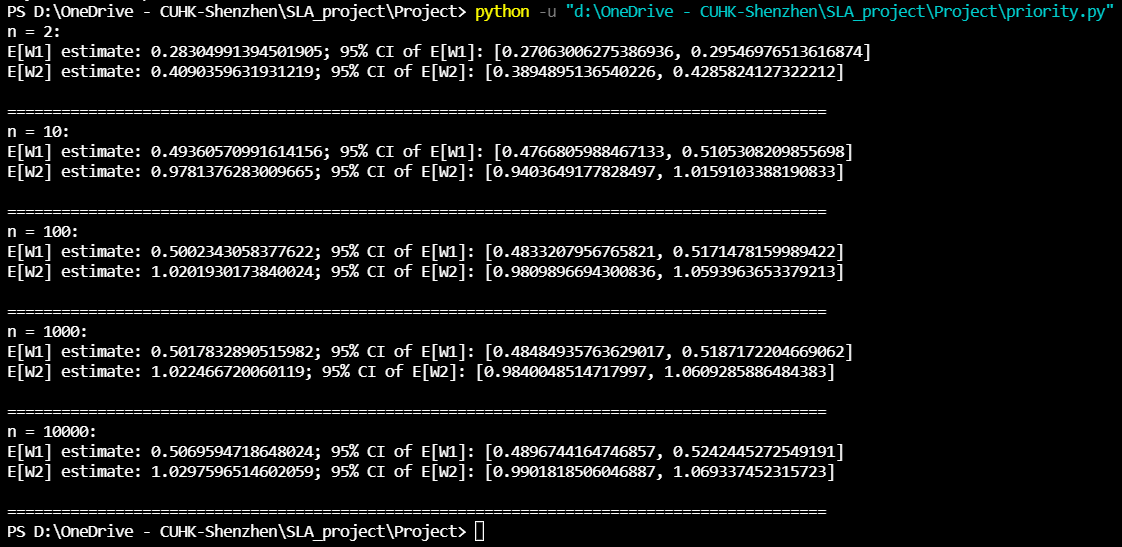
\includegraphics[height=6.4cm]{./figures/priority_result.png}
	\caption{Priority queue simulation results in python}
	\label{fig:fig2}
\end{figure}
In this setting of this two customer classes, type 1 customers have a service rate of 2 while type 2 customers have a service rate of 1. This indicates that type 1 customers generally take less time to finish their service. Indeed, it can be proved that in nonpreemptive M/G/1 systems, the \textbf{shortest-job-first (SJF)} routing principle can be proved to minimize the mean waiting time over all the customers \citep{harchol2013performance}. 	

Except for the long time it takes to estimate the waiting time expectation, the nonpreemptive policy, however, is still a poor choice even under the SJF principles. This is because the numerator contains second-moment term ${\rm E}[V^2]$, which results in huge variance especially under heavy-tail service distributions. Even for high priority customers, the mean waiting time is suffered due to the variance in the service distribution. This can be seen that a high priority customer may still be stuck behind possible ongoing low priority customers if they already start the service. Hence the ability to preempt ongoing service is important though in real world it can scarcely be satisfied. 

% \section{References}
% Koklu, M., \& Ozakan, I. A. (2020). Multiclass classification of dry beans using computer vision and machine learning techniques. \emph{Computers and Electronics in Agriculture, }174, 105507. \href{https://doi.org/10.1016/j.compag.2020.105507}{doi: https://doi.org/10.1016/j.compag.2020.105507}


% Słowiński, G. (2021). Dry beans classification using machine learning. \emph{Proceedings http://ceur-ws. org ISSN, 1613}, 0073.





% \section{Examples of citations, figures, tables, references}
% \label{sec:others}

% \subsection{Citations}
% Citations use \verb+natbib+. The documentation may be found at
% \begin{center}
% 	\url{http://mirrors.ctan.org/macros/latex/contrib/natbib/natnotes.pdf}
% \end{center}

% Here is an example usage of the two main commands (\verb+citet+ and \verb+citep+): Some people thought a thing \citep{rubinstein2004cross} but other people thought something else \citep{asmussen2007stochastic}. Many people have speculated that if we knew exactly why \citet{ross2014introduction} thought this\dots

% \subsection{Figures}
% \lipsum[10]
% See Figure \ref{fig:fig1}. Here is how you add footnotes. \footnote{Sample of the first footnote.}
% \lipsum[11]

% \begin{figure}
% 	\centering
% 	\fbox{\rule[-.5cm]{4cm}{4cm} \rule[-.5cm]{4cm}{0cm}}
% 	\caption{Sample figure caption.}
% 	\label{fig:fig1}
% \end{figure}

% \subsection{Tables}
% See awesome Table~\ref{tab:table}.

% The documentation for \verb+booktabs+ (`Publication quality tables in LaTeX') is available from:
% \begin{center}
% 	\url{https://www.ctan.org/pkg/booktabs}
% \end{center}


% \begin{table}
% 	\caption{Sample table title}
% 	\centering
% 	\begin{tabular}{lll}
% 		\toprule
% 		\multicolumn{2}{c}{Part}                   \\
% 		\cmidrule(r){1-2}
% 		Name     & Description     & Size ($\mu$m) \\
% 		\midrule
% 		Dendrite & Input terminal  & $\sim$100     \\
% 		Axon     & Output terminal & $\sim$10      \\
% 		Soma     & Cell body       & up to $10^6$  \\
% 		\bottomrule
% 	\end{tabular}
% 	\label{tab:table}
% \end{table}

% \subsection{Lists}
% \begin{itemize}
% 	\item Lorem ipsum dolor sit amet
% 	\item consectetur adipiscing elit.
% 	\item Aliquam dignissim blandit est, in dictum tortor gravida eget. In ac rutrum magna.
% \end{itemize}

\bibliographystyle{plain}
% \bibliographystyle{unsrtnat}
\bibliography{references}  %%% Uncomment this line and comment out the ``thebibliography'' section below to use the external .bib file (using bibtex) .
% \bibliography{custom}

%% Uncomment this section and comment out the \bibliography{references} line above to use inline references.
% \begin{thebibliography}{1}

% 	\bibitem{kour2014real}
% 	George Kour and Raid Saabne.
% 	\newblock Real-time segmentation of on-line handwritten arabic script.
% 	\newblock In {\em Frontiers in Handwriting Recognition (ICFHR), 2014 14th
% 			International Conference on}, pages 417--422. IEEE, 2014.

% 	\bibitem{kour2014fast}
% 	George Kour and Raid Saabne.
% 	\newblock Fast classification of handwritten on-line arabic characters.
% 	\newblock In {\em Soft Computing and Pattern Recognition (SoCPaR), 2014 6th
% 			International Conference of}, pages 312--318. IEEE, 2014.

% 	\bibitem{hadash2018estimate}
% 	Guy Hadash, Einat Kermany, Boaz Carmeli, Ofer Lavi, George Kour, and Alon
% 	Jacovi.
% 	\newblock Estimate and replace: A novel approach to integrating deep neural
% 	networks with existing applications.
% 	\newblock {\em arXiv preprint arXiv:1804.09028}, 2018.

% \end{thebibliography}


\end{document}
